\documentclass{standalone}
\usepackage{tikz}
\usetikzlibrary{patterns, positioning}


\begin{document}
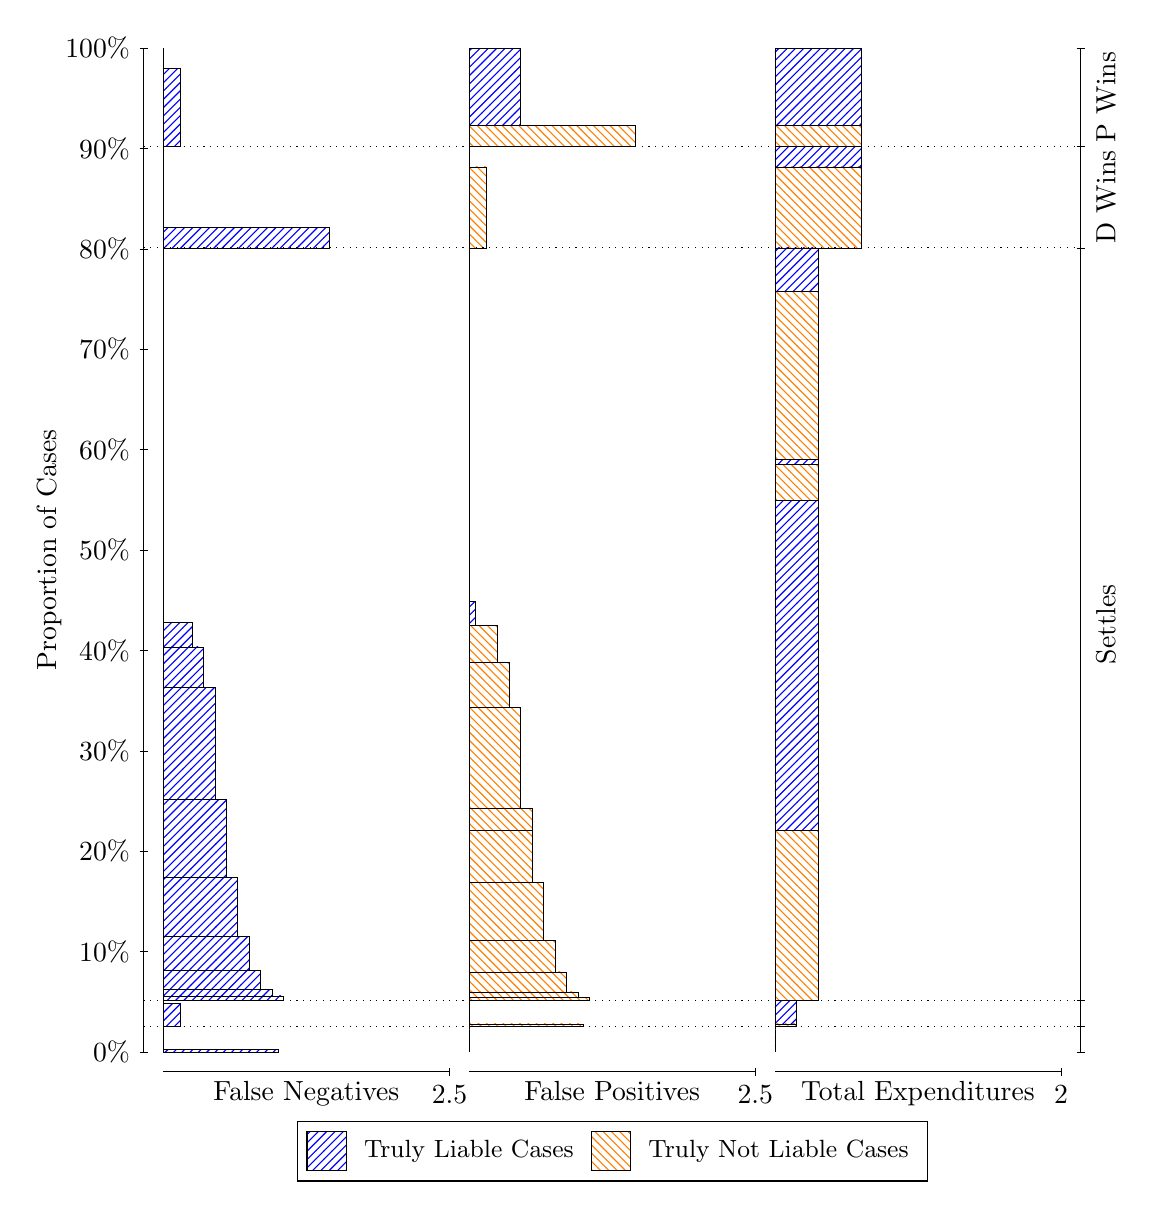
\begin{tikzpicture}
\draw[black, very thin] (1.5,1.75) -- (1.5,14.5);
\node[rotate=90, text=black, anchor=center] at (0.3, 8.125) {Proportion of Cases};
\draw[black, very thin] (1.45,1.75) -- (1.55,1.75);
\node[text=black, anchor=east] at (1.45, 1.75) {0\%};
\draw[black, very thin] (1.45,3.025) -- (1.55,3.025);
\node[text=black, anchor=east] at (1.45, 3.025) {10\%};
\draw[black, very thin] (1.45,4.3) -- (1.55,4.3);
\node[text=black, anchor=east] at (1.45, 4.3) {20\%};
\draw[black, very thin] (1.45,5.575) -- (1.55,5.575);
\node[text=black, anchor=east] at (1.45, 5.575) {30\%};
\draw[black, very thin] (1.45,6.85) -- (1.55,6.85);
\node[text=black, anchor=east] at (1.45, 6.85) {40\%};
\draw[black, very thin] (1.45,8.125) -- (1.55,8.125);
\node[text=black, anchor=east] at (1.45, 8.125) {50\%};
\draw[black, very thin] (1.45,9.4) -- (1.55,9.4);
\node[text=black, anchor=east] at (1.45, 9.4) {60\%};
\draw[black, very thin] (1.45,10.675) -- (1.55,10.675);
\node[text=black, anchor=east] at (1.45, 10.675) {70\%};
\draw[black, very thin] (1.45,11.95) -- (1.55,11.95);
\node[text=black, anchor=east] at (1.45, 11.95) {80\%};
\draw[black, very thin] (1.45,13.225) -- (1.55,13.225);
\node[text=black, anchor=east] at (1.45, 13.225) {90\%};
\draw[black, very thin] (1.45,14.5) -- (1.55,14.5);
\node[text=black, anchor=east] at (1.45, 14.5) {100\%};

\draw[black, very thin] (13.4,1.75) -- (13.4,14.5);
\draw[black, very thin] (13.35,1.75) -- (13.45,1.75);
\node[anchor=west] at (13.35, 1.75) {};
\draw[black, very thin] (13.35,2.072) -- (13.45,2.072);
\node[anchor=west] at (13.35, 2.072) {};
\draw[black, very thin] (13.35,2.4038) -- (13.45,2.4038);
\node[anchor=west] at (13.35, 2.4038) {};
\draw[black, very thin] (13.35,11.962) -- (13.45,11.962);
\node[anchor=west] at (13.35, 11.962) {};
\draw[black, very thin] (13.35,13.254) -- (13.45,13.254);
\node[anchor=west] at (13.35, 13.254) {};
\draw[black, very thin] (13.35,14.5) -- (13.45,14.5);
\node[anchor=west] at (13.35, 14.5) {};

\draw[black, very thin, pattern color=blue, pattern=north east lines] (1.75,1.75) rectangle (3.2033,1.7839);
\draw[black, very thin, pattern color=orange, pattern=north west lines] (1.75,1.7839) rectangle (1.75,2.072);
\draw[black, very thin, pattern color=blue, pattern=north east lines] (1.75,2.072) rectangle (1.968,2.369);
\draw[black, very thin, pattern color=orange, pattern=north west lines] (1.75,2.369) rectangle (1.75,2.4038);
\draw[black, very thin, pattern color=blue, pattern=north east lines] (1.75,2.4038) rectangle (3.276,2.4624);
\draw[black, very thin, pattern color=blue, pattern=north east lines] (1.75,2.4624) rectangle (3.1307,2.542);
\draw[black, very thin, pattern color=blue, pattern=north east lines] (1.75,2.542) rectangle (2.9853,2.7894);
\draw[black, very thin, pattern color=blue, pattern=north east lines] (1.75,2.7894) rectangle (2.84,3.2206);
\draw[black, very thin, pattern color=blue, pattern=north east lines] (1.75,3.2206) rectangle (2.6947,3.9698);
\draw[black, very thin, pattern color=blue, pattern=north east lines] (1.75,3.9698) rectangle (2.5493,4.9601);
\draw[black, very thin, pattern color=blue, pattern=north east lines] (1.75,4.9601) rectangle (2.404,6.381);
\draw[black, very thin, pattern color=blue, pattern=north east lines] (1.75,6.381) rectangle (2.2587,6.8958);
\draw[black, very thin, pattern color=blue, pattern=north east lines] (1.75,6.8958) rectangle (2.1133,7.2012);
\draw[black, very thin, pattern color=orange, pattern=north west lines] (1.75,7.2012) rectangle (1.75,11.962);
\draw[black, very thin, pattern color=blue, pattern=north east lines] (1.75,11.962) rectangle (3.8573,12.224);
\draw[black, very thin, pattern color=orange, pattern=north west lines] (1.75,12.224) rectangle (1.75,13.254);
\draw[black, very thin, pattern color=blue, pattern=north east lines] (1.75,13.254) rectangle (1.968,14.238);
\draw[black, very thin, pattern color=orange, pattern=north west lines] (1.75,14.238) rectangle (1.75,14.5);
\draw[black, very thin, pattern color=orange, pattern=north west lines] (5.6333,1.75) rectangle (5.6333,2.0382);
\draw[black, very thin, pattern color=blue, pattern=north east lines] (5.6333,2.0382) rectangle (5.6333,2.072);
\draw[black, very thin, pattern color=orange, pattern=north west lines] (5.6333,2.072) rectangle (7.0867,2.1068);
\draw[black, very thin, pattern color=blue, pattern=north east lines] (5.6333,2.1068) rectangle (5.6333,2.4038);
\draw[black, very thin, pattern color=orange, pattern=north west lines] (5.6333,2.4038) rectangle (7.1593,2.4433);
\draw[black, very thin, pattern color=orange, pattern=north west lines] (5.6333,2.4433) rectangle (7.014,2.5123);
\draw[black, very thin, pattern color=orange, pattern=north west lines] (5.6333,2.5123) rectangle (6.8687,2.7665);
\draw[black, very thin, pattern color=orange, pattern=north west lines] (5.6333,2.7665) rectangle (6.7233,3.1714);
\draw[black, very thin, pattern color=orange, pattern=north west lines] (5.6333,3.1714) rectangle (6.578,3.9062);
\draw[black, very thin, pattern color=orange, pattern=north west lines] (5.6333,3.9062) rectangle (6.4327,4.5617);
\draw[black, very thin, pattern color=orange, pattern=north west lines] (5.6333,4.5617) rectangle (6.4327,4.844);
\draw[black, very thin, pattern color=orange, pattern=north west lines] (5.6333,4.844) rectangle (6.2873,6.1224);
\draw[black, very thin, pattern color=orange, pattern=north west lines] (5.6333,6.1224) rectangle (6.142,6.7014);
\draw[black, very thin, pattern color=orange, pattern=north west lines] (5.6333,6.7014) rectangle (5.9967,7.1643);
\draw[black, very thin, pattern color=blue, pattern=north east lines] (5.6333,7.1643) rectangle (5.706,7.4696);
\draw[black, very thin, pattern color=blue, pattern=north east lines] (5.6333,7.4696) rectangle (5.6333,11.962);
\draw[black, very thin, pattern color=orange, pattern=north west lines] (5.6333,11.962) rectangle (5.8513,12.991);
\draw[black, very thin, pattern color=blue, pattern=north east lines] (5.6333,12.991) rectangle (5.6333,13.254);
\draw[black, very thin, pattern color=orange, pattern=north west lines] (5.6333,13.254) rectangle (7.7407,13.516);
\draw[black, very thin, pattern color=blue, pattern=north east lines] (5.6333,13.516) rectangle (6.2873,14.5);
\draw[black, very thin, pattern color=orange, pattern=north west lines] (9.5167,1.75) rectangle (9.5167,2.0382);
\draw[black, very thin, pattern color=blue, pattern=north east lines] (9.5167,2.0382) rectangle (9.5167,2.072);
\draw[black, very thin, pattern color=orange, pattern=north west lines] (9.5167,2.072) rectangle (9.7892,2.1068);
\draw[black, very thin, pattern color=blue, pattern=north east lines] (9.5167,2.1068) rectangle (9.7892,2.4038);
\draw[black, very thin, pattern color=orange, pattern=north west lines] (9.5167,2.4038) rectangle (10.062,4.5617);
\draw[black, very thin, pattern color=blue, pattern=north east lines] (9.5167,4.5617) rectangle (10.062,8.7518);
\draw[black, very thin, pattern color=orange, pattern=north west lines] (9.5167,8.7518) rectangle (10.062,9.2147);
\draw[black, very thin, pattern color=blue, pattern=north east lines] (9.5167,9.2147) rectangle (10.062,9.2732);
\draw[black, very thin, pattern color=orange, pattern=north west lines] (9.5167,9.2732) rectangle (10.062,11.413);
\draw[black, very thin, pattern color=blue, pattern=north east lines] (9.5167,11.413) rectangle (10.062,11.962);
\draw[black, very thin, pattern color=orange, pattern=north west lines] (9.5167,11.962) rectangle (10.607,12.991);
\draw[black, very thin, pattern color=blue, pattern=north east lines] (9.5167,12.991) rectangle (10.607,13.254);
\draw[black, very thin, pattern color=orange, pattern=north west lines] (9.5167,13.254) rectangle (10.607,13.516);
\draw[black, very thin, pattern color=blue, pattern=north east lines] (9.5167,13.516) rectangle (10.607,14.5);
\draw[black, dotted] (1.5,2.072) -- (13.4,2.072);
\draw[black, dotted] (1.5,2.4038) -- (13.4,2.4038);
\draw[black, dotted] (1.5,11.962) -- (13.4,11.962);
\draw[black, dotted] (1.5,13.254) -- (13.4,13.254);
\draw[black, very thin] (1.75,1.5) -- (5.3833,1.5);
\node[text=black, anchor=north] at (3.5667, 1.5) {False Negatives};
\draw[black, very thin] (5.3833,1.45) -- (5.3833,1.55);
\node[text=black, anchor=north] at (5.3833, 1.45) {2.5};

\draw[black, very thin] (5.6333,1.5) -- (9.2667,1.5);
\node[text=black, anchor=north] at (7.45, 1.5) {False Positives};
\draw[black, very thin] (9.2667,1.45) -- (9.2667,1.55);
\node[text=black, anchor=north] at (9.2667, 1.45) {2.5};

\draw[black, very thin] (9.5167,1.5) -- (13.15,1.5);
\node[text=black, anchor=north] at (11.333, 1.5) {Total Expenditures};
\draw[black, very thin] (13.15,1.45) -- (13.15,1.55);
\node[text=black, anchor=north] at (13.15, 1.45) {2};



\node[text=black, centered, rotate=90] at (13.72, 7.1827) {Settles};
\node[text=black, centered, rotate=90] at (13.72, 12.608) {D Wins};
\node[text=black, centered, rotate=90] at (13.72, 13.877) {P Wins};

\draw (7.449999999999999,1.5) node[draw=none] (baseCoordinate) {};
\begin{scope}[align=center]
        \matrix[scale=0.5, draw=black, below=0.5cm of baseCoordinate, nodes={draw}, column sep=0.1cm]{
            \node[rectangle, draw, minimum width=0.5cm, minimum height=0.5cm, pattern color=blue, pattern=north east lines] {}; &
            \node[draw=none, font=\small, text=black] (B) {Truly Liable Cases}; &
            \node[rectangle, draw, minimum width=0.5cm, minimum height=0.5cm, pattern color=orange, pattern=north west lines] {}; &
            \node[draw=none, font=\small, text=black] (B) {Truly Not Liable Cases}; \\
            };
\end{scope}

\end{tikzpicture}
\end{document}